\section{Anwedungen des Satzes von Kutta-Joukowski}
\label{joukowski:anwendungen}

\subsection{Magnus Effekt}
\begin{figure}
	\centering
	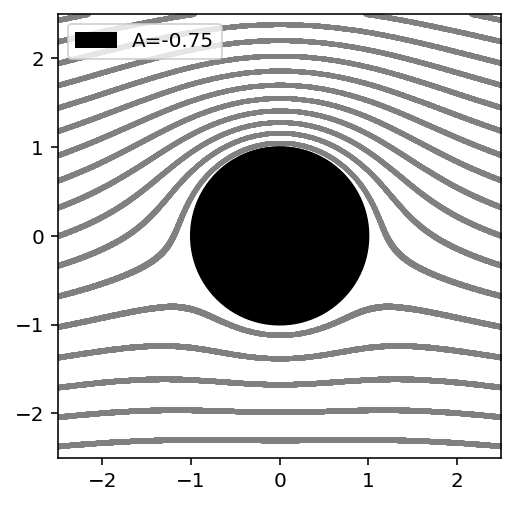
\includegraphics[width=0.45\textwidth]{papers/joukowski/images/05_stroemungslinien/Magnus_Strom_A075_g.png}
	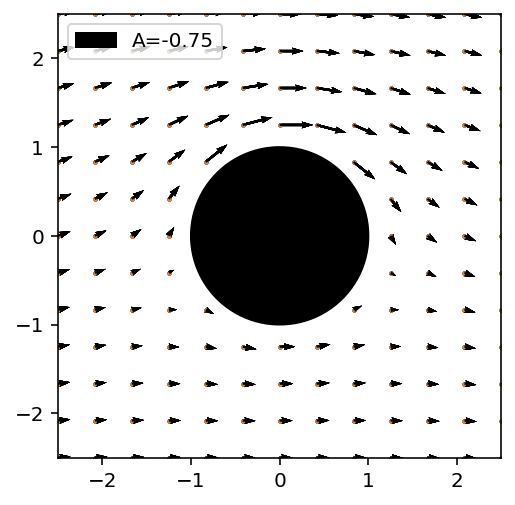
\includegraphics[width = 0.45\textwidth]{papers/joukowski/images/05_stroemungslinien/Magnus_Speed_A075.png}
\end{figure}

Bei rotierenden Zylindern entsteht eine Kraft, sofern eine Luftströmung existiert. Dieser Effekt kann beispielsweise eingesetzt werden, um den Kraftstoffverbrauch von Schiffen zu senken.

Grafisch lässt sich dieser Effekt aufzeigen, indem die Funktion $f(z)$ zu folgendem Ausdruck erweitert wird:
\begin{equation}
	\label{joukowski:Stroemungslinien:equation_magnus}
	f(z) = \frac{v_\infty}{2} \cdot \biggl(z+ \frac{1}{z}\biggr) - i\cdot A\cdot \log(z).
\end{equation}
Mit dem Parameter A kann der Effekt eines rotierenden Zylinders in einem Strömungsfeld gesteuert werden. Wird der Parameter $A$ beispielsweise auf $-0.75$ gesetzt, resultiert ein Strömungs- und Geschwindigkeitsfeld wie in Abbildung ~\eqref{joukowski:Stroemungslinien:fig_magnus}. Anhand dieser Abbildung wird intuitiv deutlich, dass eine auftriebserzeugende Kraft nach oben entsteht.

\subsection{Tragflügel}
\begin{figure}
	\centering
	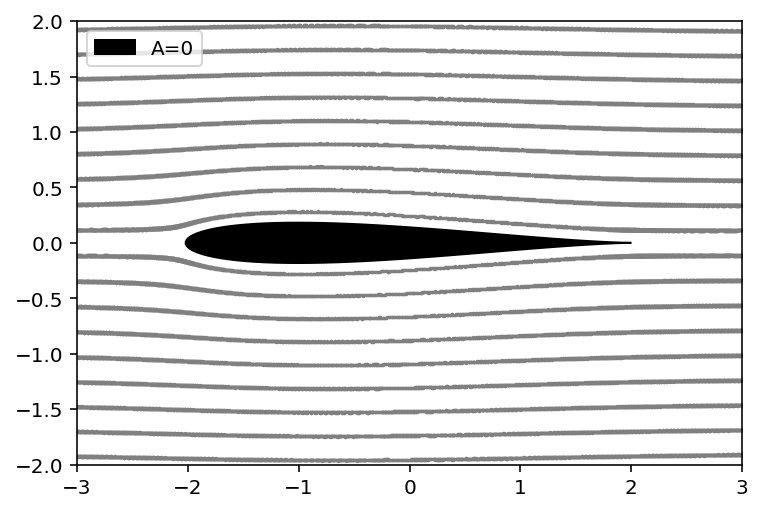
\includegraphics[width=0.6\textwidth]{papers/joukowski/images/05_stroemungslinien/fluegel_strom_A000_V04_g.png}
%	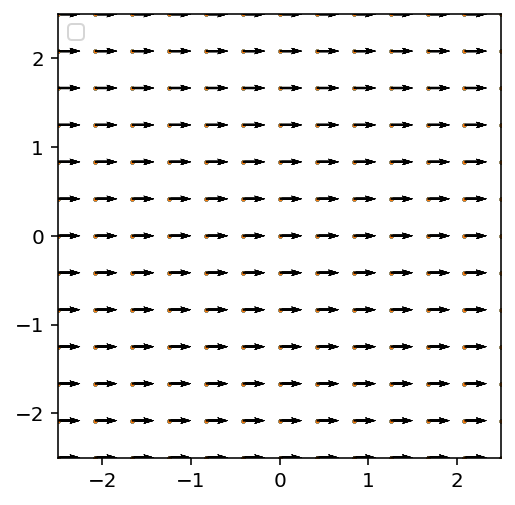
\includegraphics[width = 0.45\textwidth]{papers/joukowski/images/05_stroemungslinien/speed.png}
	\caption{
		\label{joukowski:Stroemungslinien:fig_fluegel1}
	}
\end{figure}

\begin{figure}
	\centering
	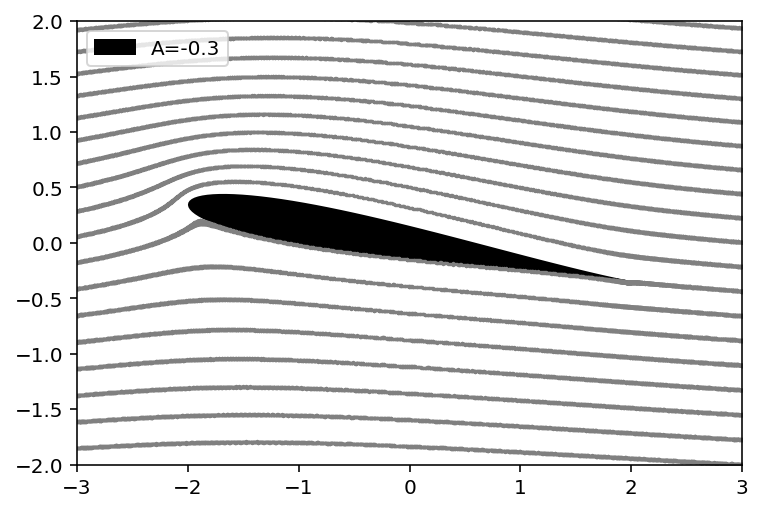
\includegraphics[width=0.6\textwidth]{papers/joukowski/images/05_stroemungslinien/fluegel_strom_A030_Rot_V02_g.png}
%	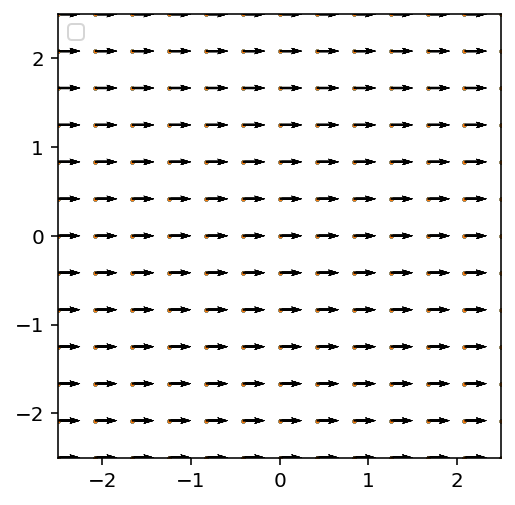
\includegraphics[width = 0.45\textwidth]{papers/joukowski/images/05_stroemungslinien/speed.png}
	\caption{
		\label{joukowski:Stroemungslinien:fig_fluegel2}
	}
\end{figure}

Nun haben wir bereits viel über Geschwindigkeiten und Strömungen gesprochen.
Die interessante Frage ist jedoch, was das alles mit einem Flügelprofil zu tun hat.
Ein Einheitskreis kann relativ einfach so transformiert werden, dass er einem an der reellen Achse symmetrischen Flügelprofil entspricht.
Hierzu braucht es lediglich eine Verschiebung mit kleinem Realanteil und anschlissend erneut die Transformation $z + \frac{1}{z}$.
Da Strömungslinien holomorph sind, können auch diese transformiert werden.
Somit kann der Einheitskreis in die gewünschte Form transformiert werden, und die Strömungslinien folgen anschliessend durch exakt dieselbe Transformation.

In Abbildung ~\eqref{joukowski:Stroemungslinien:fig_fluegel1} wird ein symmetrisches Flügelprofil gezeigt. Dieses erzeugt zunächst keinen Auftrieb und dient lediglich zu Anschauungszwecken.

Abbildung ~\eqref{joukowski:Stroemungslinien:fig_fluegel2} entspricht einem Flügelprofil mit Anstellwinkel.
Hierzu muss der transformierte Flügel in der komplexen Ebene im Uhrzeigersinn rotiert werden.~
Damit die Strömungslinien der Realität entsprechen, muss der Faktor $A$ in Gleichung ~\eqref{joukowski:Stroemungslinien:equation_magnus} passend gewählt werden. Dies haben wir numerisch mithilfe unserer Visualisierung ermittelt.
Mit diesem Modell können wir die Strömungslinien um ein Flügelprofil ermitteln.
Es wird ausserdem deutlich, dass dieser Flügel Auftrieb generieren muss, da eine Asymmetrie entsteht.

\subsection{Vom Modell zum Koeffizienten}